\section{Case study}
\label{S:w4}
We used \textit{URBANFlux system} that consists of a network of Wi-Fi detectors called OD\_Pods \cite{farooq2015ubiquitous} to record MAC addresses, signal strengths and times of connection for individual devices on four urban roads within the study area (\cref{fig:odloc}). Coverage zone of each OD\_Pod can be approximated as a sphere with a radius of 50 meters. We collected the Wi-Fi signals from different smartphones on two separate days. The first wave of data collection was done on Wednesday, June 15, 2017, from 10 A.M. to 1 P.M. in a congested area in downtown Toronto. In order to increase the size of the data, and reduce human and experimental errors, the second round of data collection was done in the same area on Wednesday, August 22, 2018, from 10 A.M. to 1 P.M.

In both data collection rounds, a congested area in downtown Toronto were selected as the case study for data collection. OD\_Pods were placed on four streets forming a loop. As it is depicted in \cref{fig:odloc}, and described in~\cite{kalatian2018mobility}, the selected streets form a grid loop with a perimeter of 857 meters. Designated streets and locations of OD\_Pods were set so as to maintain the heterogeneity of the data. The designated loop includes a mix of separate bike lanes, side-walks, arterial, two-lane and one-lane streets. In addition, north edge of the loop is on the path of Toronto's 506 Carlton streetcars. Traffic signals on all four corners of the loop make the experiment more realistic and applicable to urban areas. The sensors are placed on mid-block locations so that no overlap occurs between coverage areas of OD\_Pods.

\begin{figure}
%\begin{subfigure}{0.5\textwidth}\centering
\centering
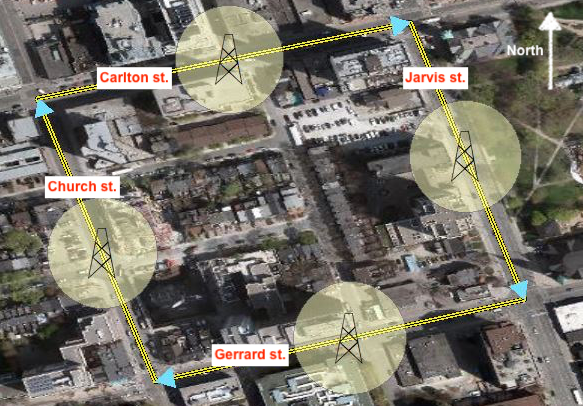
\includegraphics[scale=0.425]{chapter_2/figures/odpods.png}
\caption{Study area in downtown Toronto and OD\_Pods location}
\label{fig:odloc}
%\end{subfigure}
\end{figure}

\subsection{Data Collection}
To collect labelled data, four volunteers were assigned a mode of transportation, each going around the designated loop for 10 rounds. Volunteers were selected from our lab members, with different age categories, one female and three males, to account for heterogeneity of the data. All phones used by participants were using Android OS, including one Samsung J5, two Huawei P10 plus and one Google Pixel 2. MAC address of participants' devices are recorded by \emph{URBANFlux system}. Modes are assigned to each participant in a way to resemble the actual share of different modes in downtown Toronto. To do so, the shares of walking, biking and driving trips are set to be approximately 25\%, 25\%, and 50\%. Data recorded from movements between each two OD\_Pods are considered as a trip with their respective mode. In addition, OD\_Pods automatically track MAC addresses of all Wi-Fi enabled devices moving in the area. MAC addresses different than those of the participants, which were recorded by at least two independent OD\_Pods during the experiment, were considered as the unlabelled trips. \cref{tab:Total} represents the total number of trips for each mode, along with unlabelled trips.

\begin{table}
\centering
\label{tab:Tripsum}
\caption{Total number of trips collected for each mode}
\begin{tabular}{|l|c|}
\hline
    {\textbf{Mode}} & {\textbf{Number of Trips}} \\
\hline
\hline
{Walking} & 213  \\
{Biking} &        184     \\
{Driving} &        451     \\
{Unlabelled trips} &        1990     \\
\hline
\hline
Total & 2838\\
\hline
\end{tabular}
\label{tab:Total}
\end{table}


\subsection{Data Pre-processing}
Raw data extracted from OD\_Pods included three columns:
\begin{enumerate}
\item[a.] MAC address of a device
\item[b.] Signal strength
\item[c.] Time stamp
\end{enumerate}
All the data from different OD\_Pods are merged together. By having MAC addresses of participants, and non-participants detected by two independent OD\_Pods, connection data belonging to them are separated. A movement is considered as trip if it is detected by two consecutive OD\_Pods. Connection details from origin and destination OD\_Pods are investigated, and based on their data, 15 variables are defined as classification features. These variables are categorized to 3 groups as provided in \cref{tab:var}~\cite{kalatian2018mobility}, and discussed below:
%\begin{landscape}
\begin{table}

\caption{Details of variables defined for classification}
\scalebox{0.96}{
\begin{tabularx}{\textwidth}{|c|s|c|b|}
\hline
    {\textbf{ID}} & {\textbf{Variable}}& {\textbf{Unit}}& {\textbf{Description}}
\\
\hline
\multicolumn{4}{|l|}{\textit{Time}}\\
\hline
{1} & Relative Speed  & -&Normalized ratio of "distance with no coverage zone between two involved OD\_Pods" to its respective travel time, is used as an representation of travel speed. \\
\hline
{2} &        Connection Time: origin  & s &Time during which a device is communicating with the OD\_Pod in the origin zone. \\
\hline
{3} &        Connection Time: destination & s& Time during which a device is communicating with the OD\_Pod in the destination zone. \\
\hline
\multicolumn{4}{|l|}{\textit{Connection Number}}\\
\hline

{4} &        \# of Connections: origin &-& Number of connections between the OD\_Pod and a user's device, while a device is in the origin zone.  \\
\hline
{5} &       \# of Connections: destination & -& Number of connections between the OD\_Pod and a user's device, while a device is in the destination zone. \\
\hline
{6} &        \# of Connections: average  & - & Average of rows 4 and 5. \\
\hline
\multicolumn{4}{|l|}{\textit{Signal Strength}}\\
\hline

{7} &        Signal Variance: origin & \(\displaystyle dBm^2\) & Variance in the signal strengths of the connections to the origin OD\_Pod. \\
\hline
{8} &        Signal  Variance: destination & \(\displaystyle dBm^2\) & Variance in the signal strengths of the connections to the destination OD\_Pod.   \\
\hline
{9} &        Signal Variance: average & \(\displaystyle dBm^2\) & Average of rows 7 and 8. \\
\hline
{10} &        Signal 1st Derivative: origin & dBm/s & 1st derivative of the signal strengths of the connections to the origin OD\_Pod.    \\
\hline
{11} &        Signal 1st Derivative: destination & dBm/s& 1st derivative of the signal strengths of the connections to the destination OD\_Pod.   \\\hline
{12} &        Signal 1st Derivative: average & dBm/s  & Average of rows 10 and 11.  \\\hline
{13} &        Signal 2nd Derivative: origin & \(\displaystyle dBm/s^2\)& 2nd derivative of the signal strengths of the connections to the origin OD\_Pod.  \\\hline
{14} &        Signal 2nd Derivative: destination  & \(\displaystyle dBm/s^2\)& 2nd derivative of the signal strengths of the connections to the destination OD\_Pod. \\\hline
{15} &        Signal 2nd Derivative: average & \(\displaystyle dBm/s^2\)  & Average of rows 13 and 14.   \\\hline
\end{tabularx} }
\label{tab:var}
\end{table}
%\end{landscape}
\begin{enumerate}
\item[\textbf{a.}] \textbf{Time Variables:} Relative travel speed and connection time are included in this group:
 Speed-related variables, i.e. average, maximum and minimum speed, and their derivatives, have been the main features for classification in related literature~\cite{poucin2018activity}. However, speed alone is not adequate to predict transportation mode, as in congested areas, different transportation modes may move with similar speeds. 

\item[\textbf{b.}] \textbf{Connection Variables:} Number of connections between an OD\_Pod and a user's device, while a device is in the coverage zone. It can be intuitively expected that for users spending more time in a coverage zone, the number of connections are higher than users passing the area in shorter times.

\item[\textbf{c.}] \textbf{Signal Strength Variables:} Attributes observing the fluctuations in signal strength, i.e. variance, first and second derivative of signal strengths during the connection time. Fluctuations in signal strength are expected to be higher when a user pass through a coverage area using modes with higher pace or acceleration.
\end{enumerate}